\section{Introduction to MATLAB and R}
\paragraph{Primary Text Reading.}
\texttt{http://www.r-project.org/about.html} \\
\texttt{http://cran.r-project.org/manuals.html} \linebreak
\textit{especially} \textbf{An Introduction to R} and \textbf{R Data Import/Export}
\index{MATLAB}\index{R language}

\subsection{Statistical Computing}
Many analytical methods are highly complex, involving multiple calculations, formulas, and graphics.\footnote{A good resource for exploring more on statistical computing is the American Statistical Association website for \textbf{Statistics Computing and Graphics} at, \texttt{http://stat-computing.org/}}
Statistical computing, also known as computational statistics may also be used to refer to computationally-intensive statistical methods including resampling methods, Markov chain Monte Carlo methods, local regression, kernel density estimation and generalized additive models.

Both MATLAB and R are statistical computing environments; they both have broad support in the quantitative finance community as well as having a large number of libraries or packages that contain specialized functions. In class, we will attempt to be as platform-independent as possible, as well as trying to avoid proprietary data formats, such as Microsoft Excel. All data sets will be comma-delimited, or tab/space delimited so that they can be used by any editor and work equally well in MATLAB, R, or any other statistical software package.

\subsubsection{MATLAB}
To MATLAB, \emph{everything} is a matrix, including a single value, a \emph{scalar}. MATLAB has matrix math processing built in as well as a rich set of programming features for data access, graphical user interface, and mathematical computation and simulation. Despite its long list of features, MATLAB is very easy to use and can produce meaningful results in a short time span. MATLAB has robust file processing capability, meaning that very large datasets, perhaps amounting to millions of items, pose no difficulty. Having numerous functions already available and tested make MATLAB a good environment for rapid development of models. Writing programs in a language like C++ requires considerably more commitment of time and programming expertise.

There is a wide literature available for users of MATLAB and numerous examples of functions available through the worldwide web. There are hundreds of user contributions at MATLAB Central\footnote{The MATLAB Central File Exchange is an excellent source of code samples and ideas in various categories of MATLAB applications, \\ \texttt{http://www.mathworks.com/matlabcentral/fileexchange/loadCategory.do}}.

MATLAB has a rich set of functions for mathematics, statistics, data analysis, and graphics. Additionally, users may write their own scripts and functions in the form of \emph{M-files}, the programming language of MATLAB. 
The latest technical documentation on MATLAB is available online\footnote{\texttt{http://www.mathworks.com/access/helpdesk/help/techdoc/index.html}}. \citeA{martinez2008csh} provides an excellent resource for statistics in MATLAB.

\ecaption{Normal Probability Density Function in MATLAB}
This is an example of the Normal Probability Density Function \eqref{eq:pdf} in \textsc{MATLAB}. \emph{This is a simple example, and a more complex version already exists in the MATLAB library of functions.}\index{MATLAB}
\begin{verbatim}
     function [p] = MynormPDF(z)
     % Normal Probability Density Function
     p = 1 / sqrt(2.0 * pi) * exp(-z.^2 / 2.0);
\end{verbatim}
To call this function, entering \texttt{MynormPDF(0)} into the MATLAB Command Window would display \texttt{ans =  0.3989}.

The next example demonstrates how to read Excel workbook data into a MATLAB matrix variable, $q$. An example of the data is represented in Table~\ref{tab:matlab-xl}. The file name is \texttt{QQQQ.xls} and the data we want is in the Excel sheet named ``Daily''. Then, we will extract the first 100 items from column 2 of the dataset [1:100, 2], and calculate its standard deviation and its mean. The last line compares element [21, 2] with the 100-item mean that we just calculated. If $q[21,2]>mean(q[1:100,2])$ then it will return 1 (for \emph{true}), otherwise, it returns 0 (for \emph{false}).
\ecaption{Using MATLAB to Use Excel Workbook Data}\index{MATLAB}
\begin{verbatim}
     q=xlsread(`/filepath/data/QQQQ.xls', `Daily');
     mnth=q(1:100,2)
     std(mnth)
     mean(mnth)
     q(21,2)>mean(mnth)
\end{verbatim}

\begin{table}[htbp]
	\centering
	\begin{tabular}{rrrrrrr}
	\toprule
	\multicolumn{7}{c}{Stock Price Data Imported into MATLAB} \\
	\hline
	Date	& Open & High	& Low & Close	& Volume	& Adj. Close \\
	\hline
	38115 &	48.03 &	48.46 & 47.9 &	48.21 &	97037800	 & 48.21\\
	38114 &	48.24 &	48.7	&  48.06 & 48.4	 & 128058700	& 48.4\\
	38113 &	48.94 &	49.23 & 47.87 & 48.04 &	140008300 &	48.04 \\
	\vdots & \vdots & \vdots & \vdots & \vdots & \vdots & \vdots \\
	36959 &	37.61 &	37.67 &	37.08 &	37.52 &	97043600 &	37.14 \\
	\bottomrule
	\end{tabular}
	\caption{Stock Price Finance Data Imported into MATLAB}
	\label{tab:matlab-xl}
\end{table}

\subsubsection{R Language}
The R environment is a language for statistical computing and advanced graphics. It is a GNU project which means it can be downloaded for free.\footnote{To download the latest version of the R environment and any documentation and packages, go to \texttt{http://cran.r-project.org/}.} When we refer to the R statistical environment, for convenience we will identify it as, ``R language'' to mean the entire system of statement syntax, graphics, and packages. Two excellent learning resources are \citeA{Rmanual}, the online R documentation, and \citeA{Rbook}, which contains numerous programming examples.

To demonstrate some basic functionality, we will load a file from Ruey Tsay's teaching website, and plot a time series.\index{Tsay, Ruey}
\ecaption{Loading data from a website in R}
\begin{verbatim}
# Read in a Ruey Tsay dataset from a web page.
filename="http://faculty.chicagogsb.edu/ruey.tsay/teaching/
     fts2/d-ibmvwewsp6203.txt"
rets<-read.table(filename) 
with(rets,{retsts<-ts(V3); plot(retsts,ylab=`Returns')})
\end{verbatim}

Some of the data that we will be working with has header information, a title at the top of each column. To load these data, we simply append, \texttt{header=T}. This example loads a tab-delimited file named \texttt{intdef.txt}, generates some summary statistics, and creates the plot in Figure~\ref{figure:intdef}.
\index{read.table@\texttt{read.table} (in R)}
\begin{verbatim}
# Read a data file with a header.
intrt<-read.table(`intdef.txt', header=T)
summary(intrt)
with(intrt,sd(i3))
with(intrt,plot(year,i3))
\end{verbatim}

\begin{figure}[t]
  \centering
  \includegraphics[scale=.5]{intdef}
  \caption{Interest Rate Time Series Plot in R}
  \label{figure:intdef}
\end{figure}

For a simple side-by-side comparison of some basic functions of both MATLAB and R, see Table~\ref{tab:matlab-r-funcs}.
\begin{table}[htbp]
	\centering
	\begin{tabular}{lll}
	\toprule
	Function & MATLAB & R \\
	\hline
	Expansion & Toolboxes & Packages \\
	Programming & M code & R code \\
	File Input & \texttt{load} & \texttt{read.table} \\
	Getting Help & \texttt{help plot} & \texttt{?plot} \\
	Matrices & rows, then columns & columns, then rows \\
	Change Directory & \texttt{cd(`/path')} & \texttt{setwd(`/path')} \\
	\bottomrule
	\end{tabular}
	\caption{Basic Functions in MATLAB and R}
	\label{tab:matlab-r-funcs}
\end{table}

\subsection{Loading Data}
\paragraph{MATLAB.} There are a few ways to load data. The easiest is \texttt{load}\index{load@\texttt{load} (in MATLAB)}. To create an array variable name \texttt{plainTS} from a single-column text file \texttt{plain.txt}, we need the statement,
\ecaption{Loading single-column text file in MATLAB}
\begin{verbatim}
plainTS=load(`/path/plain.txt');
\end{verbatim}

The semicolon at the end of the statement suppresses any output to the screen. Leaving out the semicolon would display each line of text as it read into MATLAB. If our data set had multiple columns which were separated by spaces or tabs, we could use the same syntax, and we would still have a single variable, but with multiple columns. To refer to a single item in the array, such as the 27th observation, we address it \texttt{plainTS(27)}. If we had multiple columns, we want to refer to column 2, we simply use \texttt{plainTS(:,2)}.

Importing delimited data sets requires \texttt{dlmread}\index{dlmread@\texttt{dlmread} (in MATLAB)}, and is not much more difficult. To read only the numerical data from the five-column  tab-delimited file, \texttt{SP-MidCap4.txt}
\ecaption{Loading multiple-column tab-delimited text file in MATLAB}
\begin{verbatim}
sp_mid=dlmread(`/path/SP-MidCap4.txt', `\t', 0, 1);
\end{verbatim}
The \texttt{`\textbackslash t'} is the delimiter, which in our case is the tab character. To use comma-delimited text, we replace that with `,' or whichever marker we require. We can specify the starting column and row number of the data. MATLAB uses a zero-based index, so to get \emph{all rows} but columns 1 to whichever is the last column, we enter 0 and 1, respectively. Once loaded, we have a variable named \texttt{sp\_mid}. To refer to the 120th row, and 3rd column data item, \texttt{sp\_mid(120,3)}.

Now try to load \texttt{SP-MidCap.csv} which is comma-delimited and has the first row consisting of column names. We do not want to import the first column, which are non-numerical dates, nor do we want the column names, since they too are non-numerical.
\ecaption{Loading multiple-column comma-delimited text file in MATLAB}
\begin{verbatim}
sp_mid=dlmread(`/path/SP-MidCap.csv', `,', 1, 1);
\end{verbatim}

There are other methods in MATLAB for loading data and writing results back to a file, but these two will work fine for most purposes. We have also only concerned ourselves with numerical data at this point. We address date conversions in Section~\ref{date-handling}.

\paragraph{R Environment.} Just as we explored one method of loading tab-delimited data and one method for comma-delimited data in MATLAB, we will discuss two ways in the R environment. One advantage is that we may load column names with our data, something we are unable to do in MATLAB. We will load all data, \emph{including column names}, from the five-column  tab-delimited file, \texttt{SP-MidCap3.txt} using \texttt{read.table}.\index{read.table@\texttt{read.table} (in R)}
\ecaption{Loading multiple-column tab-delimited text file in R}
\begin{verbatim}
mid400<-read.table(`/path/SP-MidCap3.txt', header=T)
\end{verbatim}

\pagebreak
We have two ways of using the column names from a data set. The first method is easier, but can result in name collision when multiple data sets are loaded.
\marginpar{\begin{small}\begin{flushleft}\textcolor{blue}{Name collision is the result of two processes or data sets using the same name.}\end{flushleft}\end{small}}
Now that we have \texttt{SP-MidCap3.txt} stored into a variable named \texttt{mid400}, we can assign columnn names using \texttt{attach(mid400)}\index{attach@\texttt{attach} (in R)}.
To see the names assigned to columns, we can use \texttt{names(mid400)}\index{names@\texttt{names} (in R)}.

We can refer directly to the column of data by its name, such as when we want the mean of the column \texttt{Close}, by typing \texttt{mean(Close)}. The problem is that these column names are global, which is generally a bad idea in the event that we want other data with the same name.

The second method of using the column names from a data set is preferred, and is only slightly more complex.  We do not use the \texttt{attach} statement, but instead refer to a column by variable name and column name using \texttt{with}\index{with@\texttt{with} (in R)}. We can compute the mean of the column \texttt{Close}, by typing \texttt{with(mid400, mean(Close))}.
We still have the column names in the variable, and we can view the first row of data by typing \texttt{mid400[1,]}.

Reading comma-separated data is as easy as reading table data -- the tab or space delimited files we just discussed. This time, we use the statement, 
\texttt{read.csv}\index{read.csv@\texttt{read.csv} (in R)}.
\ecaption{Loading multiple-column comma-delimited text file in R}
\begin{verbatim}
mid400<-read.csv(`/path/SP-MidCap.csv', header=T)
\end{verbatim}
Once the data set is loaded, all functions work exactly the same as before.

\subsection{Date Handling}\label{date-handling}\index{Epoch Date}
\paragraph{Date Formatting.} Most computer systems store a date as the number of days or number of minutes since a specific date.
\marginpar{\begin{small}\begin{flushleft}\textcolor{red}{Be aware of the computer epoch date of the system you import and export into.}\end{flushleft}\end{small}}
Some Unix systems store the date as number of days since January 1, 1970, while some software may use a different date. This ``epoch date'' may cause confusion when reading and writing dates into a statistical package. For instance, what is the date value of 733671? That depends on which system created that date. This particular date value came from MATLAB, where it represents September 20, 2008, but in Excel (with 1904 Date System enabled) it is September 21, 3912, and it is September 20, 3908 with 1904 Date System disabled.

The spreadsheet software in OpenOffice for X11 uses a date value of 1 for December 31, 1899 (\emph{which is technically January 0, 1900}), but Microsoft Excel uses January 1, 1904, the Lotus 1-2-3 ``standard.'' In Excel, the ``1904 Date System'' can be turned off, so that date value of 1 becomes January 1, 1900.

\paragraph{MATLAB.} Dates must be stored as numbers in MATLAB, which measures the number of days since January 1, 0. There are functions to convert a string date into a number. For example the date, 20 September 2008, could be entered a few ways, such as,
\index{datenum@\texttt{datenum} (in MATLAB)}
\begin{verbatim}
my_date=datenum(`2008-09-20', `yyyy-mm-dd')
my_date=datenum(`20-Sep-2008')
\end{verbatim}
which stores the number 733671 in the variable \texttt{my\_date}. This makes date arithmetic easier, but, that number does not tell us much once stored since we like seeing months, days, and years. We can convert that number to a date string using \texttt{datestr(my\_date)}.\index{datestr@\texttt{datestr} (in MATLAB)} If we want the month, day, and year as a number, we have \texttt{[yr,mo,day]=datevec(my\_date)}\index{datevec@\texttt{datevec} (in MATLAB)}, which populated three variables as described in the left-hand side.

\paragraph{R Environment.} Our data set \texttt{mid400} has a column named \texttt{Date} which is formatted \texttt{yyyy-mm-dd}. This works well for date conversion and performing date arithmetic. To convert the item into a ``time'' data type, we need \texttt{as.POSIXlt}\index{as.POSIXlt@\texttt{as.POSIXlt} (in R)} 
so that converting the date in column 1, row 1 is done by \texttt{as.POSIXlt(mid400[1,1])}. To add 7 days to that date is as easy as \texttt{as.POSIXlt(mid400[1,1]) + (24*60*60*7)}.

R also has a full set of objects that can display and manipulate dates.
\begin{verbatim}
today<-Sys.Date()
next.week<-today+7
format(next.week, "%d %b %Y")
\end{verbatim}

\subsection{Statistical Operations}
\paragraph{MATLAB.}
There is a wide variety of statistical functions available in MATLAB. As a very brief introduction, we will look at some basic descriptive statistics. Using our \texttt{sp\_mid} data set, we compute the mean and standard deviation of the set, using \texttt{mean} and \texttt{std}, respectively. We can summarize the entire data set, column-by-column with \texttt{mean(sp\_mid)}, which returns a matrix that has one row, and has a mean for each column.

If, for example, we want the standard deviation of the most recent 200 opening prices (column 1 of the data), we need to specify the range using \texttt{std(sp\_mid(1:200, 1))}.

\paragraph{R Environment.}
There is also an extensive variety of statistical functions available in R. As a very brief introduction, we will look at some basic descriptive statistics. Using our \texttt{mid400} data set, we compute the mean and standard deviation of the set, using \texttt{mean} and \texttt{sd}, respectively. We can summarize the entire data set, column-by-column with \texttt{mean(mid400)}, which returns the mean for each column, except for \texttt{Date}, which is not numeric.

If, for example, we want the standard deviation of the most recent 200 opening prices (column 2 of the data), we need to specify the range using \texttt{sd(mid400[1:200, 2])}.

\subsection{Functions}
\paragraph{MATLAB.} Sometimes, the built-in functionality of MATLAB is not enough to handle specific requirements. In order to extend the environment, users may write functions. Here is an example of a simple moving average.
\ecaption{Moving Average Function in MATLAB}
\begin{verbatim}
function y = movavg(x,p)
% Simple Moving Average written as a MATLAB demo
% by Andrew P. Acosta
% This works with a COLUMN of numbers only.
y=zeros(size(x));
for n=p:size(x,1)
    y(n)=mean(x(n-p+1:n));
end
\end{verbatim}

The elements of a function are the word \texttt{function} as the first keyword, followed by the variable(s) returned by the function. A MATLAB function can return more than one variable, provided that the list is enclosed in brackets (\textit{e.g.} \texttt{[x,y,z]}). Comments in MATLAB begin with a percent sign (\texttt{\%}). The contents of the comments placed between the first line of the function and the first line of instructions will display when a user types \texttt{help} followed by the function name. It is a good way of documenting user-defined code.

What follows is the actual work of the function. The return variable(s) must be set somewhere in this segment. The three-day moving average for the first ten observations is called by, \texttt{movavg(sp\_mid(1:10,1), 3)}.


\paragraph{R Environment.} Since R also is a programming language, there is a specific syntax for writing functions. Here is an example of a simple moving average.
\ecaption{Moving Average Function in R}
\begin{verbatim}
movavg<-function(x,p) { 
    # Simple Moving Average written as an R demo 
    # by Andrew P. Acosta
    y<-numeric(length(x))
    for(n in p:length(x)) {
        y[n]<-mean(x[(n-p+1):n])
        }
    y
}
\end{verbatim}

The elements of a function are the word \texttt{function} after assignment to the return variable. Comments in R begin with a pound or hash symbol sign (\texttt{\#}). 

What follows is the actual work of the function. The return variable must be set somewhere in this segment. The three-day moving average for the first ten observations is called by, \texttt{movavg(mid400[1:10,2], 3)}.

\subsection{Graphing}
\begin{figure}[tbh]
  \centering
  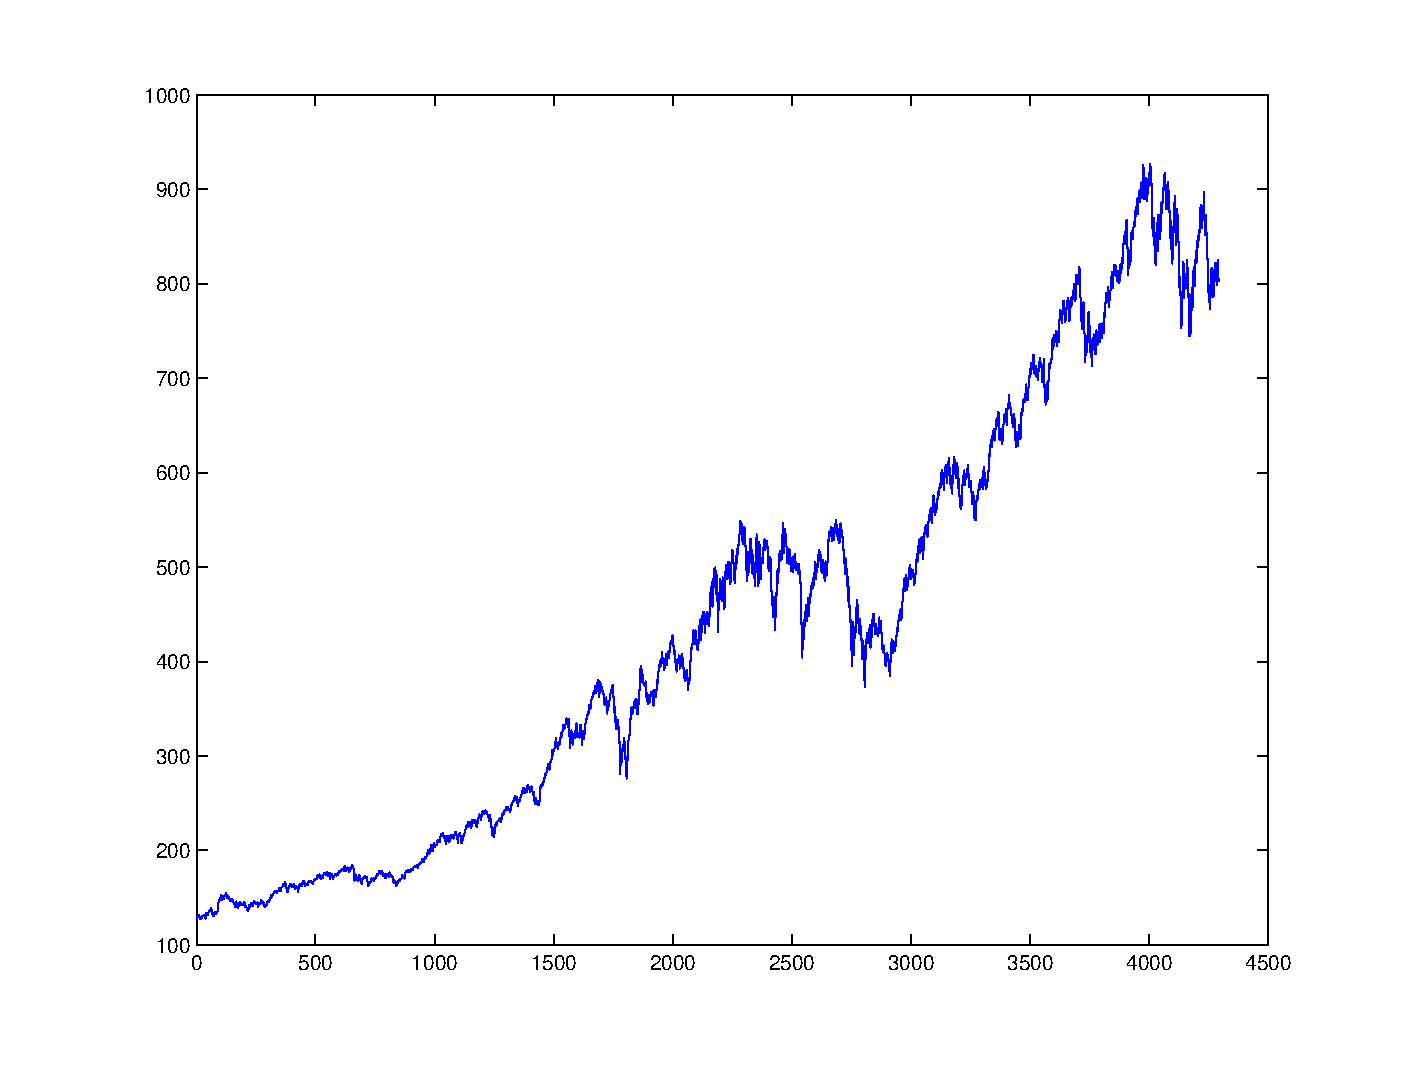
\includegraphics[scale=.5]{sp_mid}
  \caption[\texttt{SP-MidCap-sort.csv} Data Set in MATLAB]{Plot of \texttt{SP-MidCap-sort.csv} Data Set using MATLAB statement \texttt{plot(sp\_mid(:,1))}.}
  \label{figure:spmid}
\end{figure}
\paragraph{MATLAB.} There is an extensive collection of graphical features in MATLAB.  One of the most used functions is \texttt{plot}\index{plot@\texttt{plot} (in MATLAB)}, which creates an X,Y plot which is depicted in Figure~\ref{figure:spmid}.

To work with the data set as a MATLAB time series, we will explore the \texttt{timeseries}\index{timeseries@\texttt{timeseries} (in MATLAB)} and \texttt{tscollection}\index{tscollection@\texttt{tscollection} (in MATLAB)} objects. 

\paragraph{R Environment.} It is no surprise that R also has an extensive collection of graphical feaures.  One of the most used functions is \texttt{plot}\index{plot@\texttt{plot} (in R)}, which creates an X,Y plot which is depicted in Figure~\ref{figure:mid400}.
\begin{figure}[tbh]
  \centering
  \includegraphics[scale=.6]{mid400}
  \caption[\texttt{SP-MidCap-sort.csv} Data Set in R]{Plot of \texttt{SP-MidCap-sort.csv} Data Set using R programming. \linebreak \texttt{with(mid400, plot(Open, type="l", col="red", ylab="Open", main="S\&P 400 Midcap"))}.}
  \label{figure:mid400}
\end{figure}

To work with the data set as an R time series, we will explore the \texttt{ts}\index{ts@\texttt{ts} (in R)} object. 

\pagebreak
\subsection{Technical Issues}
As with any data, there could be some level of work required to ``clean'' the data, or to make it presentable for analysis.  This cleanup effort will depend greatly upon the quality and source of the data, as well as the type of analysis and software.

Some issues arise at the source of \fts{} data, and generally become typical problems solved through information technology. Often, they are simple matters of parsing a text file, rearranging rows and columns, or validating source data. Such rudimentary tasks, as well as more complex pre-analytical text formatting, are solved by scripting languages like Perl\index{Perl Language} or Python\index{Python Language}.

Be aware that some \fts{} data may have the most recent data first, yet your graphics and numerical analysis expects oldest data first. In this case, you simply need to reverse the order of the observations in the data set.

Some data conversion is more complicated. For example, if a process is receiving XML\index{XML}-formatted data, it is worth knowing how the data are described by the format. The same applies to reading and writing HTML\index{HTML} data. MATLAB and R have capabilities of handling formatted data, but it is still important to know the underlying formatting issues.

In other cases, there may be missing data, or data that are simply incorrect. How would you react to a price series such as \{23.38, 26.73, \textbf{95.69}, 26.55, 26.47, 26.63\}? Do you explain the 95.69 that seems to be out of place? Does it belong there? Is it an error? How do you know? How do you locate these kinds of numbers in a large data set?

Even if the data is correct on some superficial level, there remain several other issues such as: of normalizing a variable's range, proper sampling methods, and capturing patterns. \citeA{pyle1999dpd} writes in detail about these concerns as well as many others.

No doubt, you will encounter errors in data, or require them to be modified in some way before or after your analysis. Being able to do this is vital, and the responsibility should not be relegated to a lesser importance.